% ****** Start of file apssamp.tex ******
%
%   This file is part of the APS files in the REVTeX 4.2 distribution.
%   Version 4.2a of REVTeX, December 2014
%
%   Copyright (c) 2014 The American Physical Society.
%
%   See the REVTeX 4 README file for restrictions and more information.
%
% TeX'ing this file requires that you have AMS-LaTeX 2.0 installed
% as well as the rest of the prerequisites for REVTeX 4.2
%
% See the REVTeX 4 README file
% It also requires running BibTeX. The commands are as follows:
%
%  1)  latex apssamp.tex
%  2)  bibtex apssamp
%  3)  latex apssamp.tex
%  4)  latex apssamp.tex
%
\documentclass[%
%reprint,
%superscriptaddress,
%groupedaddress,
%unsortedaddress,
%runinaddress,
%frontmatterverbose, 
preprint,
%preprintnumbers,
onecolumn,
notitlepag,
%nofootinbib,
%nobibnotes,
%bibnotes,
 amsmath,amssymb,
 aps,
 pra,
%prb,
%rmp,
%prstab,
%prstper,
%floatfix,
]{revtex4-2}

\usepackage{graphicx}% Include figure files
\usepackage{dcolumn}% Align table columns on decimal point
\usepackage{bm}% bold math
\usepackage{bbm}%bold symbols
\usepackage{hyperref}% add hypertext capabilities
\usepackage[tickmarkheight=0.1cm]{todonotes}
\usepackage{soul}
\usepackage{url}
\usepackage{cleveref}
\usepackage{natbib}
\usepackage{showkeys}% shows citation keys	
\usepackage[draft,inline,nomargin]{fixme} 
\fxsetup{theme=color} %Para hacer comentarios y resaltarlos con colores.
\FXRegisterAuthor{cv}{acv}{CV}

%%% MACROS 

\newcommand{\be}{\begin{equation}}
\newcommand{\ee}{\end{equation}}
\newcommand{\ben}{\begin{equation*}}
\newcommand{\een}{\end{equation*}}
\newcommand{\tr}{\mbox{Tr}} 
\providecommand{\abs}[1]{\lvert#1\rvert}                                    
\newcommand{\bra}[1]{\ensuremath{\langle #1 |}}
\newcommand{\ket}[1]{\ensuremath{| #1 \rangle}}
\newcommand{\prj}[1]{\ensuremath{| #1 \rangle \langle #1 |}}
\newcommand{\ovl}[2]{\ensuremath{\langle #1 | #2 \rangle}}
\newcommand{\matel}[3]{\ensuremath{\langle #1 | #2 | #3 \rangle}}
\newcommand{\expval}[2]{\ensuremath{\langle{#1}\rangle_{#2}}}
\begin{document}
%\preprint{}
\title[]{Reaction coordinate and quantum trjectories}
\author{Luis Eduardo Herrera}
\email{leherrerar@unal.edu.co }
\affiliation{Departamento de Física, Universidad Nacional de Colombia, Carrera 30 No.45-03, Bogotá, Colombia.}
\author{Carlos Viviescas}
\email{clviviescasr@unal.edu.co }
\affiliation{Departamento de Física, Universidad Nacional de Colombia, Carrera 30 No.45-03, Bogotá, Colombia.}
\begin{abstract}
\todo[inline]{Write the abstract at the end}
\end{abstract}
	
\maketitle
%------------------------------------------------------------
%
\section{Introduction}
\todo[inline]{Write the introduction at the end}
\section{Spin-boson model}
In the first part of the this notes we closely follows Gernot \todo[]{Add a reference to Gernots notes on quantum transport.}
We consider a single two-level system (TLS) linearly coupled to a bosonic environment, 
\begin{equation}
H = \frac{\omega}{2} \sigma_{z}+\sum_{k} \frac{t_{k}^{2}}{\omega_{k}} S^{2}+S \sum_{k} t_{k}\left(a_{k}+a_{k}^{\dagger}\right)+\sum_{k} \omega_{k} a_{k}^{\dagger} a_{k}.
\end{equation}
Here, $a_{k}$ and $a^{\dagger}_{k}$ are bosonic anihilation and creation operators of the environment mode $k$, with frequency $\omega_{k}$, satisfying $[b_{k},b^{\dagger}_{k'}] = \delta_{kk'} \mathbbm{1}$, and $S$ is the coupling operator acting on the system and accounting for its interaction with all modes of the envirionment through coupling amplitudes $t_{k}$, which without loss of generality are chosen to be real. The environment spectral density is then $J^{(0)} = \sum_{k} t_{k}^2 \delta (\omega -  \omega_{k})$.
In this notes we shall consider the two cases $S = \sigma_{z}$, the pure-dephasing limit, and $S = \sigma_{x}$, the dissipative spin-boson model. For both models $S^2 =1$ and the renormalization becomes a trivial shift.
\subsection{Reaction coordinate mapping}
We map the system \todo[]{Talk about the Bogoliubov transforms} into a model where a collective mode of the environment, the reaction coordinate (RC), denoted by the creation (annihilation) operator $b$ ($b^{\dag}$), is incorporated into an effective system Hamiltonian coupled to a residual environment \todo[]{Luis: please write the appendix explaining how to get the reaction coordinate}(see Appendix~\ref{A:RCmap}). The spin-boson hamiltonian decomposes into
\begin{equation}
H = H_{S} + H_{B} + H_{I},
\end{equation}
with system Hamiltonian
\begin{equation}
H_{\text{S}}=\frac{\omega}{2} \sigma^{z}+\Omega_{0}\left(b^{\dagger}+\frac{g}{\Omega_{0}} S\right)\left(b+\frac{g}{\Omega_{0}} S\right)+ \Omega_{0} \Delta (b + b^{\dag})^{2},
\end{equation}
where the coupling strength and the energy of the RC are obtained via
\begin{equation}
g^{2}=\frac{1}{2 \pi \Omega_{0}} \int_{0}^{\infty} \omega J^{(0)}(\omega) d \omega, 
\quad
\Omega_{0}^{2}=\frac{\int_{0}^{\infty} \omega J^{(0)}(\omega) d \omega}{\int_{0}^{\infty} \frac{J^{(0)}(\omega)}{\omega} d \omega},
\end{equation} 
and the system renormalization is given by
\begin{equation}
\Omega_{0} \cdot \Delta \equiv \sum_{k} \frac{h_{k}^{2}}{\Omega_{k}}=\frac{1}{2 \pi} \int_{0}^{\infty} \frac{J^{(0)}(\omega)}{\omega} d \omega.
\end{equation}
The residual environment, with creation (annihilation) operators $b_{k}$ ($b_{k}^{\dag}$),  has hamiltonian
\begin{equation}
H_{B}= \sum_{k} \Omega_{k}\ b_{k}^{\dagger} b_{k}, 
\end{equation}
and is characterized by its spectral density
\begin{equation}
J^{(1)}(\omega) \equiv 2 \pi \sum_{k} h_k^2 \delta(\omega-\Omega_k) = \frac{4 g^{2} J^{(0)}(\omega)}{\left[\frac{1}{\pi} \mathcal{P} \int \frac{J^{(0)}\left(\omega^{\prime}\right)}{\omega-\omega^{\prime}} d \omega^{\prime}\right]^{2}+\left[J^{(0)}(\omega)\right]^{2}}.
\end{equation}
It couples only to the RC through the interaction hamiltonian
\begin{equation}
H_{I} = (b + b^{\dag}) \sum_{k} h_{k} (b_{k} + b_{k}^{\dagger}). 
\end{equation}
\subsection{Lindblad master equation and quantum trajectories}
We now assume the environment is only weakly coupled to the residual environment, and threat it within a Lindblad master equation for the reduced state of the composite TLS and RC system (see Appendix~\ref{B:LME}),
\begin{equation}
\label{eq:LME}
\dot{\rho}(t) = -i [H_{S}, \rho(t)] + \mathcal{D}[\sqrt{\gamma} b] \rho + \mathcal{D}[\sqrt{\bar{\gamma}} b^{\dag}] \rho \equiv \mathcal{L}\rho,
\end{equation}
where $\mathcal{D}[J]\rho \equiv J\rho J^{\dag} - \frac{1}{2} J^{\dag} J \rho - \frac{1}{2}  \rho J^{\dag} J \rho$, and we assumed that only the residual environment is in thermal equilibrium during the whole evolution. 
Instead of directly solving \eqref{eq:LME} we consider particular diffusive unravelings of it. Assuming a continuous monitoring of the residual environment with perfectly efficiency, the state of the system will evolve conditioned on the measurement record according to the diffusive stochastic master equation
\begin{equation}
d\rho_{c} = \mathcal{L}\rho_{c} \, dt +  \mathcal{H}[d\xi_{1}\,\sqrt{\gamma} b] \rho_{c} +  \mathcal{H}[d\xi_{2}\, \sqrt{\bar{\gamma}} b^{\dag}] \rho_{c},
\end{equation} 
where $\mathcal{H}[J] \rho \equiv  J \rho + \rho J^{\dag} - \tr [J \rho + \rho J^{\dag}] \rho$.  The complex Wiener process $d\boldsymbol{\xi} = (d\xi_{1}, d\xi_{2})^{\top}$ has vanishing ensemble average, $E[d\boldsymbol{\xi}] = 0$, with correlations 
\begin{equation}
d\boldsymbol{\xi} d\boldsymbol{\xi}^{\dag} = \mathbbm{1} dt, \quad  d\boldsymbol{\xi} d\boldsymbol{\xi}^{\top} = \mathsf{Y} dt.
\end{equation}
Here $\mathbbm{1}$ is the identity matrix and $\mathsf{Y}$ is a $2 \times 2$ complex symmetric matrix. Physical choices of $\mathsf{Y}$ are restricted by the condition that the $4 \times 4$ correlation matrix $U$ for the real vector $(\text{Re}\, d\boldsymbol{\xi} ,\text{Im} d\boldsymbol{\xi} )^{\top}$,
\be
\mathsf{U} = \frac{1}{2} \begin{pmatrix} \mathbbm{1} + \mathrm{Re}\mathsf{Y} & \mathrm{Im}\mathsf{Y}  \\ \mathrm{Im}\mathsf{Y} & \mathbbm{1} - \mathrm{Re}\mathsf{Y}  \end{pmatrix},
\ee
is positive definite. Associated with each unraveling is the measurement record upon which the evolution of $\rho_{c}$ is conditioned,  represented by the  the complex currents
\begin{equation}
\mathbf{y} \, dt  = 
\begin{pmatrix}
\langle \sqrt{\gamma}b + \mathsf{Y}_{11} \sqrt{\gamma}b^{\dag} +  \mathsf{Y}_{12} \sqrt{\bar{\gamma}} b \rangle \\
\langle \sqrt{\bar{\gamma}}b^{\dag} + \mathsf{Y}_{21} \sqrt{\gamma}b^{\dag} +  \mathsf{Y}_{22} \sqrt{\bar{\gamma}} b \rangle
\end{pmatrix} dt +
 d\boldsymbol{\xi}
\end{equation}
where each component represents a specific detection event.
We now turn to the application of our ideas to two specific cases.
\section{Applications}
We now turn to the application of our ideas to two specific cases. 
\cite{IlesSmith:2014db}
\subsection{Pure dephasing}
In this section we consider 
Let us take a two-level system, or qubit, described by the Pauli spin operator σz, and model the environment as a collection of bosonic field modes. In practice, such fields can yield an appropriate effective description even if the actual environment looks quite differently, in particular if the environmental coupling is a sum of many small contributions.2 What is fairly non-generic in the present model is the type of coupling between system and environment, which is taken to commute with the system Hamiltonian.
\appendix
\section{The reaction coordinate mapping}
\label{A:RCmap}

We desire to find a map that will render Hamiltonian \eqref{Caldeira Leggett} in the form (up to a shift):

\begin{equation}
\begin{aligned}
H &=H_{S}+\Omega_{0}\left(b^{\dagger}+\frac{g}{\Omega_{0}} S\right)\left(b+\frac{g}{\Omega_{0}} S\right)+\sum_{k} \Omega_{k}\left(b_{k}^{\dagger}+\frac{h_{k}}{\Omega_{k}}\left(b+b^{\dagger}\right)\right)\left(b_{k}+\frac{h_{k}}{\Omega_{k}}\left(b+b^{\dagger}\right)\right) \\
&=H_{S}+\Omega_{0} b^{\dagger} b+g S\left(b+b^{\dagger}\right)+\frac{g^{2}}{\Omega_{0}} S^{2}+\sum_{k} \frac{h_{k}^{2}}{\Omega_{k}}\left(b+b^{\dagger}\right)^{2}+\left(b+b^{\dagger}\right) \sum_{k} h_{k}\left(b_{k}+b_{k}^{\dagger}\right)+\sum_{k} \Omega_{k} b_{k}^{\dagger} b_{k}
\end{aligned}
\label{H tranform}
\end{equation}


where  the $b_k^{\dagger} (b_k)$ are the  creation (annihilation) operator for the new bosonic bath with modes frequencies $\Omega_k$, which are coupled linearly with the  system with strength $H_k$ and fulfill the bosonic commutation relations $ [ b_k , b_{k'}^{\dagger} ] = \delta_{k,k'}  $. 

The schematic vio of this transformations is sketched ind figure \ref{Rc_mapping_skecth}, where initaly  the system $H_s$  is coupled to all of defrees of freemod of the enviorement: The Tranformatios allos the system to interact only with a colective mode (Reaction Coordiante) of the environment, and the mode will be coupled to the residual modes of the bath.

To achieve this purpose, we apply a Bogoliubov transformation, where the annihilation operators $a_k$ are linearly transformed into  new modes $b_k$: 


\begin{figure}[!h]
\centering
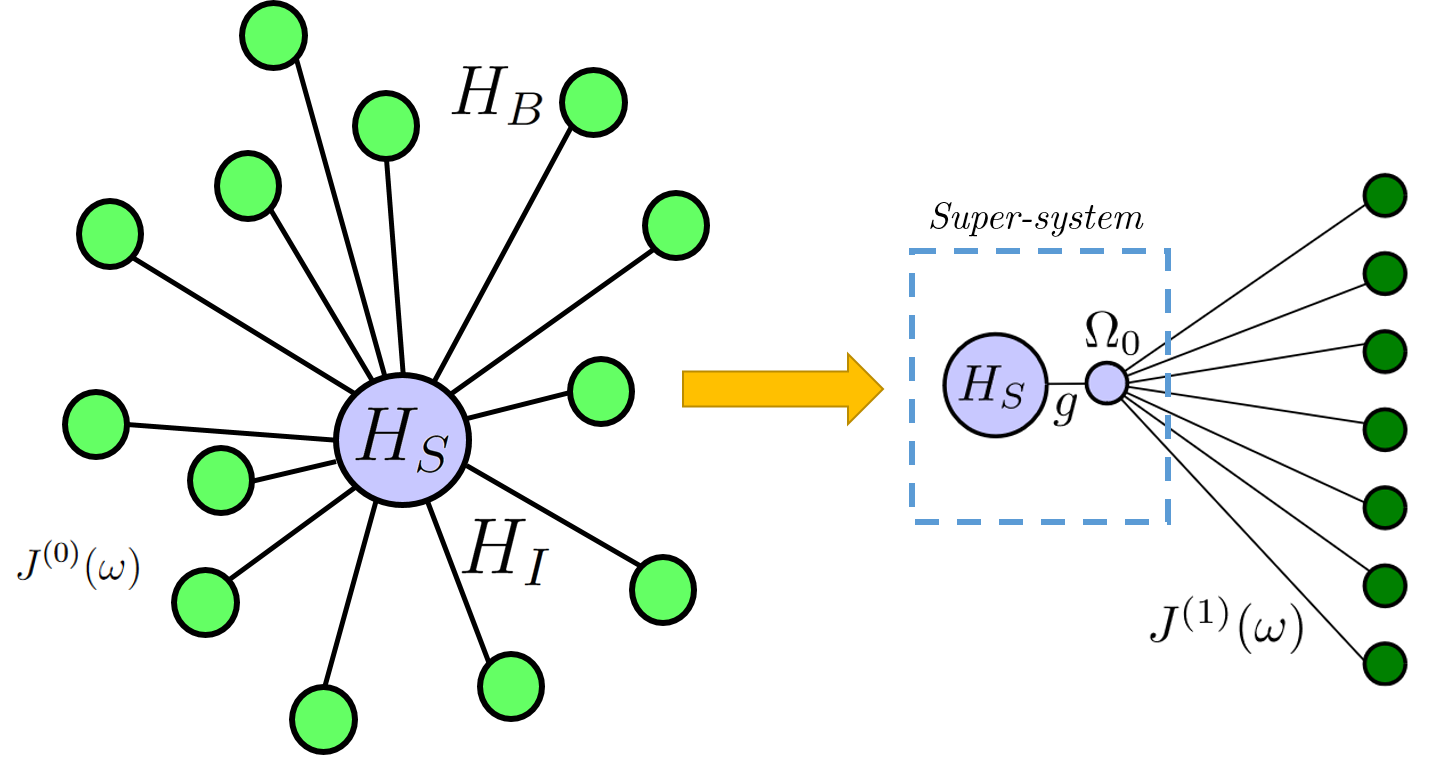
\includegraphics[width=0.9\linewidth]{Images/Rc_mapping_skecth.png}
\caption{Schematic representation of the Reaction coordinate mapping.  An original system is coupled to all of the degrees of freedom of the environment (green dots) characterivia by  a spectral density $J^{(0)}(\omega)$, after the Reaction coordinate mapping the System only couples to the collective mode(RC), and the Rc to the residual enviorement. We call the system $+$ the RC a new "supersystem" that will coueples to a new envioerment described by anew spectral desity $J^{(1)}(\omega)$. }
\label{Rc_mapping_skecth}
\end{figure}

\begin{equation}
   a_k = u_{k1} b_0 +\sum_{q\neq 0} u_{kq} b_q + v_{k0} b_0^{\dagger}+ \sum_{q\neq 0} v_{kq} b_q^{\dagger}.
\end{equation}
The distinction is made with respect $b_1$ because this mode will be selected as the reaction coordinate $(b=b_0 , b^{\dagger} = b^{\dagger}_0 )$. In order to preserve the bosonic commutation relations, the Bogoliubov transformation should be sympletic, i.e. the matrices $\mathbf{U}$  and $ \mathbf{V}$ with complex coefficients $u_kq$ and  $v_kq$ respectively obey  $\mathbf{U}\mathbf{U}^{\dagger}- \mathbf{V}\mathbf{V}^{\dagger}= \mathbb{I}$ and $\mathbf{U}\mathbf{U}^T-\mathbf{V}\mathbf{U}^T= \mathbf{0} $. The construction of the sympletic transformation can be done with an orthogonal transformation such the matrices elements are \textbf{citarr notas gernots}:
\begin{equation}
    u_{kq} = \frac{1}{2} \left( \sqrt{ \frac{\omega_k}{\Omega_q}} + \sqrt{ \frac{\Omega_q}{\omega_k}}  \right) \Lambda_{kq}, \hspace{2cm}  v_{kq} = \frac{1}{2} \left( \sqrt{ \frac{\omega_k}{\Omega_q}} - \sqrt{ \frac{\Omega_q}{\omega_k}}  \right) \Lambda_{kq},
\label{orthogonal}
\end{equation}
where $\omega_k$ and $\Omega_k$} are real valued and the $\Lambda_{kq}$ satisfy

\begin{equation}
    \sum_q \Lambda_{kq} \Lambda_{k'q} = \delta_{k,k'}
    \label{ortohonal condition}
\end{equation}


%%% Why some tranformation are sympletics and others are unitary, why the diference, what is conserved in each case, which condition ins bigger.  

The spectral density for the new bath, following the convention, is

\begin{equation}
    J^{(1)} (\omega) = 2\pi \sum_k \abs{h_k}^2 \delta (\omega- \Omega_k).
\end{equation}

In order to determine $\Lambda$, we first notice that for this bosonic map (phonon mapping) we can choose $\Lambda > 0 $, since a phase in the $b_k$ can be introduced leading to a phase change in the $h_k$ coefficient; in the same fashion we $t_k$ can be define to be a real value coefficient.

We now apply the transformation to each term in Hamiltonian \eqref{Caldeira Leggett}. Fist we tranform the interaction Hamiltonian: 

\begin{equation}
    S \sum_k \left( t_k a_k + t_k ^*a_k^{\dagger} \right) =  S \sum_k t_{k} \left[ (u_{k0} + v_{k0}) (b + b^{\dagger}) +\sum_{q\neq 0} (u_{kq} + v_{kq}) (b_{q} + b_{q}^{\dagger}) \right],
\end{equation}
where we chose $t_{k}$ real. Comparing with the linear term in $S$ of equation \eqref{H tranform}
 show that the first column of the orthogonal transformation has to be chosen as $ g \Lambda_{k 0}=t_{k} \sqrt{\frac{\omega_{k}}{\Omega_{0}}}$ and usign condition \eqref{ortohonal condition}:   


\begin{subequations}
\begin{equation}
    \sum_{k} t_{k} (u_{k0} + v_{k0}) = \sum_{k} t_{k} \sqrt{\frac{\omega_{k}}{\Omega_{0}}} \Lambda_{k0} =  g, \qquad \text{for } q=0,
\end{equation}
\begin{equation}
    \sum_{k} t_{k} (u_{kq} + v_{kq}) = \sum_{k} h_{k} \sqrt{\frac{\omega_{k}}{\Omega_{q}}} \Lambda_{kq} \equiv 0, \qquad \text{for } q\neq 0,
\end{equation}
\end{subequations}
yielding  to: 
\begin{equation}
    S \sum_k \left( t_k a_k + t_k ^*a_k^{\dagger} \right) = g  S  (b + b^{\dagger}).
\end{equation}







We follow by considering environment Hamiltonian . It transforms to : 
\begin{multline}
\hspace{7.5cm} \sum_k \omega_k a_k^{\dagger} a_k  =\\
\sum_k \omega_k  \left[ u_{k0} b^{\dagger} +\sum_{q\neq 0} u_{kq} b_q^{\dagger} + v_{k0} b+ \sum_{q\neq 0} v_{kq} b_q \right] \left[ u_{k0} b_0 +\sum_{q\neq 0} u_{kq} b_q + v_{k0} b_0^{\dagger}+ \sum_{q\neq 0} v_{kq} b_q^{\dagger} \right].
\label{third term}
\end{multline}
We look first into terms in \eqref{third term} that are independent of the RC:
\begin{multline}
\sum_{k} \omega_{k} \left[\sum_{q,q' \neq 0} \left( u_{kq } u_{kq' }  b_{q'}^{\dagger} b_q + u_{kq' } v_{kq }  b_{q'}^{\dagger} b_q^{\dagger}  + v_{kq' } u_{kq }  b_{q'} b_q + v_{kq' } v_{kq }  b_{q'} b_q ^{\dagger}\right) \right] = \\  \sum_{k} \omega_{k} \left\{ \sum_{q,q' \neq 0}  \left[    \left(  u_{kq } u_{kq' }+ v_{kq } v_{kq' }  \right) b_{q'}^{\dagger} b_q +  u_{kq'} v_{kq} \left(  b_{q'}^{\dagger} b_q^{\dagger}  +  b_q b_{q'}  \right) + v_{kq'} v_{kq} \delta_{qq'} \right] \right\},
\label{terms wihtout rc}
\end{multline}
where we used the commutation relations for the new modes, $[b_q,b_{q'}^{\dagger}] =\delta_{qq'}$. 



From parameterisation  \eqref{orthogonal} and the orthogonality of $\Lambda$, we obtain
\begin{subequations}
\label{eq:rel1}
\begin{equation}
\sum_{k} \omega_{k} u_{kq'} u_{kq} = \frac{1}{4} \Omega_{q} \delta_{q q'} + \frac{1}{4\sqrt{\Omega_{q}\Omega_{q'}}}\sum_{k} \left[ \omega_{k}^2 + \omega_{k} (\Omega_{q} + \Omega_{q'}) \right] \Lambda_{kq}\Lambda_{kq'},
\end{equation}
\begin{equation}
\sum_{k} \omega_{k} v_{kq'} v_{kq} = \frac{1}{4} \Omega_{q} \delta_{q q'} + \frac{1}{4\sqrt{\Omega_{q}\Omega_{q'}}}\sum_{k} \left[ \omega_{k}^2 - \omega_{k} (\Omega_{q} + \Omega_{q'}) \right] \Lambda_{kq}\Lambda_{kq'},
\end{equation}
\begin{equation}
\sum_{k} \omega_{k} u_{kq'} v_{kq} = - \frac{1}{4} \Omega_{q} \delta_{q q'} + \frac{1}{4\sqrt{\Omega_{q}\Omega_{q'}}}\sum_{k} \left[ \omega_{k}^2 + \omega_{k} (\Omega_{q} - \Omega_{q'}) \right] \Lambda_{kq}\Lambda_{kq'}.
\end{equation}
\end{subequations}

Demanding that the new coordinates (operators) are in normal form, 
\begin{equation}
    \sum_k  \omega_k \sum_{q,q' \neq 0}   \left(  u_{kq } u_{kq' }+ v_{kq } v_{kq' }  \right) b_{q'}^{\dagger} b_q = \sum_{q \neq 0} \Omega_q  b_{q}^{\dagger} b_q,
\end{equation}
for $q \neq 0$ and $q' \neq 0$, leads to the condition 
\begin{equation}
    \sum_{k} \omega_{k}^2 \Lambda_{kq} \Lambda_{kq'} = \Omega_{q}^{2} \delta_{qq'}.
    \label{cond1}
\end{equation}
Relations \eqref{eq:rel1} reduce to 
\begin{subequations}
\label{eq:rel2}
\begin{equation}
\sum_{k} \omega_{k} u_{kq'} u_{kq} = \frac{1}{2} \Omega_{q} \delta_{q q'} + \frac{(\Omega_{q} + \Omega_{q'})}{4\sqrt{\Omega_{q}\Omega_{q'}}}\sum_{k} \omega_{k}  \Lambda_{kq}\Lambda_{kq'},
\end{equation}
\begin{equation}
\sum_{k} \omega_{k} v_{kq'} v_{kq} = \frac{1}{2} \Omega_{q} \delta_{q q'} - \frac{(\Omega_{q} + \Omega_{q'})}{4\sqrt{\Omega_{q}\Omega_{q'}}}\sum_{k}  \omega_{k} \Lambda_{kq}\Lambda_{kq'},
\end{equation}
\begin{equation}
\sum_{k} \omega_{k} u_{kq'} v_{kq} = \frac{(\Omega_{q} - \Omega_{q'}) }{4\sqrt{\Omega_{q}\Omega_{q'}}}\sum_{k}  \omega_{k} \Lambda_{kq}\Lambda_{kq'}.
\end{equation}
\end{subequations}

where last equation is zero if one take into account the summations over $q$ and $q'$. Then  
the terms in \eqref{third term} that are independent of the RC transforms as:

\begin{multline}
    \sum_{k} \omega_{k} \left[\sum_{q,q' \neq 0} \left( u_{kq } u_{kq' }  b_{q'}^{\dagger} b_q + u_{kq' } v_{kq }  b_{q'}^{\dagger} b_q^{\dagger}  + v_{kq' } u_{kq }  b_{q'} b_q + v_{kq' } v_{kq }  b_{q'} b_q ^{\dagger}\right) \right] =\sum_{q\neq 0}  \Omega_{q} b_{q}^{\dagger} b_{q} 
    \label{eq:R1}
\end{multline}
%%%%This term should be cero 

where we have drooped the term related with the commutator since is a simple shift.

Let us now turn our attention to the terms in \eqref{third term} that depend on the RC: 



\begin{multline}
\sum_{k}\omega_{k}\left[
u_{k0} u_{k0} b^{\dagger} b + u_{k0} v_{k0} b^{\dagger} b^{\dagger} +
 v_{k0} u_{k0} b b + v_{k0} v_{k0} b b^{\dagger} + \sum_{q \neq 0 } \left( u_{k0 } u_{kq } b^{\dagger} b_q \right. \right. \\ 
 \left. \left. + u_{k0 } v_{kq } b^{\dagger} b_q^{\dagger} + v_{k0 } u_{kq } b b_q + v_{k0 } v_{kq } b b_q^{\dagger} +  u_{k0 } u_{kq } b_q^{\dagger} b + v_{k0 } u_{kq } b_q^{\dagger} b^{\dagger} + u_{k0} v_{kq } b_q b + v_{k0 } v_{kq } b_q b^{\dagger}\right)
     \right] = \\
     \sum_{k}\omega_{k}\left\{ (u_{k0}^2 + v_{k0}^2) b^{\dagger} b + u_{k0} v_{k0} (b^{\dagger} b^{\dagger} + b b) + v_{k0}^2 \right.\\ 
     \left. + \sum_{q \neq 0 }\left[ (u_{k0 } u_{kq } + v_{k0 } v_{kq})( b^{\dagger} b_{q} + b_{q}^{\dagger} b)+ (u_{k0} v_{kq} + v_{k0} u_{kq}) ( b^{\dagger} b_{q}^{\dagger} + b b_{q}) \right]\right\},
\end{multline}
where for the right hand side of the equation we used the commutation relation $[b,b^{\dagger}] = 1$. Now adding an subtracting a  term $2  u_{k0} v_{k0} b^{\dagger} b $ and writing also as $2  u_{k0} v_{k0} b^{\dagger} b =  u_{k0} v_{k0} b^{\dagger} b+ u_{k0} v_{k0}b b^{\dagger} + u_{k0} v_{k0}  $, we can complete the squares:

\begin{equation}
\begin{array}{c}
\sum_{k} \omega_{k}\left\{\left(u_{k 0}-v_{k 0}\right)^2 b^{\dagger} b+u_{k 0} v_{k 0}\left(b^{\dagger}+b \right)^2 \right. \\
\left.+\sum_{q \neq 1}\left[\left(u_{k 0} u_{k q}+v_{k 0} v_{k q}\right)\left(b^{\dagger} b_{q}+b_{q}^{\dagger} b\right)+\left(u_{k 0} v_{k q}+v_{k 0} u_{k q}\right)\left(b^{\dagger} b_{q}^{\dagger}+b b_{q}\right)\right]\right\}
\end{array}
\end{equation}



Using  the definitions \eqref{orthogonal} we have
\begin{align}
     \sum_{k} \omega_{k} (u_{k0} - v_{k0})^2= \Omega_0
\end{align}

Defininig the new coulpling strngh as:

\begin{equation}
    h_{k} \equiv \frac{1}{2\sqrt{\Omega_{0} \Omega_{q}}} \sum_{k} \omega_{k}^{2} \Lambda_{k0}\Lambda_{kq},
\end{equation}
and using the identity:

\begin{equation}
\sum_k \omega_k u_{k0} v_{k0}= \sum_{k \neq 0} \frac{\omega_{k}^{2}}{4 \Omega_{0}}- \frac{\Omega_0}{4} = \sum_{k \neq 0} \frac{h_k^{2}}{\Omega_k}
\end{equation}
yields to:


\begin{equation}
\sum_{k} \omega_{k}\left[ \left(u_{k 0}-v_{k 0}\right)^2 b^{\dagger} b+u_{k 0} v_{k 0}\left(b^{\dagger}+b \right)^2 \right]   = \Omega_{0} b^{\dagger} b +   \sum_{k \neq 0} \frac{h_k^{2}}{\Omega_k} \left(b^{\dagger}+b \right)^2
 \label{eq:R2}
\end{equation}

For the quadratic terms in $b$ and $b^{\dagger}$, and 
\begin{multline}
 \sum_{k}\omega_{k} \sum_{q \neq 1 }\left[ (u_{k0 } u_{kq } + v_{k0 } v_{kq})( b^{\dagger} b_{q} + b_{q}^{\dagger} b)+ (u_{k0} v_{kq} + v_{k0} u_{kq}) ( b^{\dagger} b_{q}^{\dagger} + b b_{q}) \right] =\\ 
 (b + b^{\dagger}) \sum_{q\neq 0} (h_{q} b_{q}^{\dagger} + h_{q} b_{q}) 
 \label{eq:R3}
\end{multline}
for the linear terms in $b$ and $b^{\dagger}$.
From results in \eqref{eq:R1}, \eqref{eq:R2}, and \eqref{eq:R3}, equation \eqref{third term} can be rewritten as
\begin{equation}
    \sum_{k} \omega_{k} a_{k}^{\dagger} a_{k} = \Omega_{0} b^{\dagger} b +     \sum_{k \neq 0} \frac{h_k^{2}}{\Omega_k} \left(b^{\dagger}+b \right)^2
    + (b + b^{\dagger}) \sum_{q\neq 0} h_q ( b_{q}^{\dagger} + b_{q}) +  \sum_{q\neq 0} \Omega_{q} b_{q}^{\dagger} b_{q}.
\end{equation}

We can further finish the mapping by setting: 

\begin{equation}
    \frac{g^{2}}{\Omega_{0}}= \sum_{k=0} \frac{t_k ^2}{\omega_k}.
\end{equation}

\begin{equation}
\Omega_{0} \cdot \Delta \equiv \sum_{k} \frac{h_{k}^{2}}{\Omega_{k}}
\end{equation}

Then 

In order to perform the transformation, we usually have to specify the matrix elements of $\Lambda$, but in this case the spectral density give the tools to perform the transformation.  The value of new coupling strength  $g$  and the RC frequency  $\Omega$ are related with the original spectral density: 

\begin{equation}
\Omega_{0}^{2}=\frac{\int_{0}^{\infty} \omega J^{(0)}(\omega) d \omega}{\int_{0}^{\infty} \frac{J^{(0)}(\omega)}{\omega} d \omega}, \quad g^{2}=\frac{1}{2 \pi \Omega_{0}} \int_{0}^{\infty} \omega J^{(0)}(\omega) d \omega .
\end{equation}

and renormalization energy $\Delta$ in terms of the new spectral density: 
\begin{equation}
    \Delta =\frac{1}{2 \Omega_0 \pi} \int_{0}^{\infty} \frac{J^{(1)}(\omega)}{\omega} d \omega
\end{equation}

The only unknown lefts terms are the new coupling constants $h_k$ and the new frequencies $\Omega_k$, this information come form the new spectral density:

\begin{equation}
    J^{(1)} (\omega) =2 \pi \sum_k |t_k|^2 \delta(\omega-\Omega_k)
\end{equation}

The relation between  the new spectral density  with the old one is found by mean of the manipulation of the Heisenberg equation of motion of the Hamiltonian, as show as follow:

\section{Transformation of the Spectral density}

The equation of motion for an operator $A$ is given by the Heisenberg equation of motion $ \dot{\boldsymbol{A}} =i \left[ \boldsymbol{ H } , \boldsymbol{A} \right] =e^{+\mathrm{i} H t}\left[H, A_{S}\right] e^{-\mathrm{i} H t} $  , where $H$ is the original Hamiltonian and blond sysmblos stand for the Hieseber pictire i.e. $  \boldsymbol{ A } = e^{+\mathrm{i} H t} A e^{-\mathrm{i} H t} $ . Then for the Hamiltonian \eqref{original system}: 

\begin{equation}
\dot{\boldsymbol{A}}=\mathrm{i} \boldsymbol{S}_{\mathbf{1}}+\mathrm{i} \boldsymbol{S}_{2} \sum t_{k}\left(\boldsymbol{a}_{\boldsymbol{k}}+\boldsymbol{a}_{\boldsymbol{k}}^{\dagger}\right)
\end{equation}


remembering that any operator of the system commute with the creation and annihilation operator of the bath, ans where we had call: 
\begin{equation}
\begin{aligned}
&\boldsymbol{S}_{1}=e^{+\mathrm{i} H t}\left[H_{S}+\sum_{k} \frac{t_{k}^{2}}{\omega_{k}} S^{2}, A\right] e^{-\mathrm{i} H t} \\
&\boldsymbol{S}_{2}=e^{+\mathrm{i} H t}[S, A] e^{-\mathrm{i} H t}
\end{aligned}
\end{equation}



For the evolution of the creation and annihilation operator we have:



\begin{equation}
\begin{aligned}
\dot{\boldsymbol{a}}_{k} &=-\mathrm{i} \omega_{k} \boldsymbol{a}_{k}-\mathrm{i} t_{k} \boldsymbol{S} \\
\boldsymbol{a}_{k}^{\dagger} &=+\mathrm{i} \omega_{k} \boldsymbol{a}_{k}^{\dagger}+\mathrm{i} t_{k} \boldsymbol{S}
\end{aligned}
\end{equation}


Now we take the Fourier Transform $\mathfrak{F} [...] = \int [...] \exp{+izt} \; dt $ with the conventios $\mathfrank{I} z > 0 $, leading to an algebraic problem. We recall the properties of the fourrien tranform of a time derivaives, and the convolution theorem: 

\begin{equation}
\mathfrak{F} [\dot{A}]   =   \int \frac{dA(t)}{d t}  e^{izt} dt =iz A(z)
\end{equation}

\begin{equation}
 \mathfrak{F} [AB] =   \int A(t) \times B(t) e^{izt} dt = \frac{1}{2\pi} \int A(z') B(z-z') dz'
\end{equation}
we get:
\begin{equation}
izA(z)= i S_1 (z) + \frac{i}{2\pi} \int S_2(z') \sum_k h_k a(z-z')+ h_k^* a^{\dagger} (z-z') dz
\label{evolution operator FT}
\end{equation}

\begin{equation}
    iza_k(z) = -i\omega_k a_k(z) - ih_k S(z)
\end{equation}


\begin{equation}
    iz\bar{ a_k} (z) = +i\omega_k \bar{ a_k}(z) + ih_k S(z)
\end{equation}

where we have denoted with a bar the Fourier transform of the adjoin operator- We can find $a_k$ and $\bar{ a_k}$ in terms of $S(z)$ from the last 2 equations  and insert in \ref{evolution operator FT}. We have then: 


\begin{equation}
izA(z)= i S_1 (z) + \frac{i}{2\pi} \int S_2(z') \sum_k |t_k|^2 \left[ \frac{1}{z-z'-\omega_k} - \frac{1}{z-z'+\omega_k} \right]  S(z-z') dz
\label{evolution operator FT final}
\end{equation}

We follow the same procedure for the transformed Hamiltonian \eqref{H tranform} and find the equation of motion:  



\begin{equation}
\begin{aligned}
\boldsymbol{ \dot{A} }&=\mathrm{i} \boldsymbol{ S_{1}}+\mathrm{i} \boldsymbol{S}_{2} g\left(\boldsymbol{b}+\boldsymbol{b}^{\dagger}\right), \\
\boldsymbol{b} &=-\mathrm{i} \Omega_{0} \boldsymbol{b}-\mathrm{i} g \boldsymbol{S}-2 \mathrm{i} \sum_{k} \frac{h_{k}^{2}}{\Omega_{k}}\left(\boldsymbol{b}+\boldsymbol{b}^{\dagger}\right)-\mathrm{i} \sum_{k} h_{k}\left(\boldsymbol{b}_{\boldsymbol{k}}+\boldsymbol{b}_{\boldsymbol{k}}^{\dagger}\right) \\
\dot{\boldsymbol{b}}^{\dagger} &=+\mathrm{i} \Omega_{0} \boldsymbol{b}^{\dagger}+\mathrm{i} g \boldsymbol{S}+2 \mathrm{i} \sum_{k} \frac{h_{k}^{2}}{\Omega_{k}}\left(\boldsymbol{b}+\boldsymbol{b}^{\dagger}\right)+\mathrm{i} \sum_{k} h_{k}\left(\boldsymbol{b}_{\boldsymbol{k}}+\boldsymbol{b}_{\boldsymbol{k}}^{\dagger}\right) \\
\dot{\boldsymbol{b}}_{\boldsymbol{k}} &=-\mathrm{i} h_{k}\left(\boldsymbol{b}+\boldsymbol{b}^{\dagger}\right)-\mathrm{i} \Omega_{k} \boldsymbol{b}_{\boldsymbol{k}} \\
\dot{\boldsymbol{b}}_{\boldsymbol{k}}^{\dagger} &=+\mathrm{i} h_{k}\left(\boldsymbol{b}+\boldsymbol{b}^{\dagger}\right)+\mathrm{i} \Omega_{k} \boldsymbol{b}_{k}^{\dagger}
\end{aligned}
\end{equation}

and apply the Fourier transform: 

\begin{equation}
\begin{aligned}
 \mathrm{i} z A(z) &\left.= \mathrm{i} S_{1}(z)+\frac{\mathrm{i} }{2 \pi} \int S_{2}\left(z^{\prime}\right) g\left[b\left(z-z^{\prime}\right)+\bar{b}\left(z-z^{\prime}\right)\right]\right) d z^{\prime} \\
z b(z) &=-\Omega_{0} b(z)-g S(z)-2 \sum_{k} \frac{h_{k}^{2}}{\Omega_{k}}[b(z)+\bar{b}(z)]-\sum_{k} h_{k}\left[b_{k}(z)+\bar{b}_{k}(z)\right] \\
z \bar{b}(z) &=+\Omega_{0} \bar{b}(z)+g S(z)+2 \sum_{k} \frac{h_{k}^{2}}{\Omega_{k}}[b(z)+\bar{b}(z)]+\sum_{k} h_{k}\left[b_{k}(z)+\bar{b}_{k}(z)\right] \\
z b_{k}(z) &=-h_{k}[b(z)+\bar{b}(z)]-\Omega_{k} b_{k}(z) \\
z \bar{b}_{k}(z) &=+h_{k}[b(z)+\bar{b}(z)]+\Omega_{k} \bar{b}_{k}(z)
\end{aligned}
\end{equation}

Using last 2 equation we can find:

\begin{equation}
b_{k}(z)=\frac{-h_{k}}{z+\Omega_{k}}[b(z)+\bar{b}(z)], \quad \bar{b}_{k}(z)=\frac{+h_{k}}{z-\Omega_{k}}[b(z)+\bar{b}(z)]
\end{equation}


and use it to to find: 


\begin{equation}
\left[\frac{z^{2}}{\Omega_{0}}-\Omega_{0}-4 \sum_{k} \frac{h_{k}^{2}}{\Omega_{k}}-4 \sum_{k} \frac{h_{k}^{2} \Omega_{k}}{z^{2}-\Omega_{k}^{2}}\right][b(z)+\bar{b}(z)]=2 g S(z)
\end{equation}


witch allow us to find the Fourier transform of the operator $A$ withe the transformed Hamiltonian. 

\begin{equation}
\begin{aligned}
 \mathrm{i} z A(z) &=\mathrm{i} S_{1}(z)+\frac{\mathrm{i} g}{2 \pi} \int S_{2}\left(z^{\prime}\right)\left[b\left(z-z^{\prime}\right)+\bar{b}\left(z-z^{\prime}\right)\right] d z^{\prime} \\
&=\mathrm{i}  S_{1}(z)+\frac{2 \mathrm{i} g^{2}}{2 \pi} \int S_{2}\left(z^{\prime}\right)\left[\frac{1}{\frac{\left(z-z^{\prime}\right)^{2}}{\Omega_{0}}-\Omega_{0}-4 \sum_{k} \frac{h_{k}^{2}}{\Omega_{k}}-4 \sum_{k} \frac{h_{k}^{2} \Omega_{k}}{\left(z-z^{\prime}\right)^{2}-\Omega_{k}^{2}}}\right] S\left(z-z^{\prime}\right) d z^{\prime}
\end{aligned}
\label{evolution operator FT final_rc}
\end{equation}



Now we can compare equation \eqref{evolution operator FT final} and  \eqref{evolution operator FT final_rc}  to find a relation between the 2 spectral densities: 

\begin{equation}
\sum_{k} t_{k}^{2}\left[\frac{1}{z-z^{\prime}-\omega_{k}}-\frac{1}{z-z^{\prime}+\omega_{k}}\right]=\frac{2 g^{2}}{\frac{\left(z-z^{\prime}\right)^{2}}{\Omega_{0}}-\Omega_{0}-4 \sum_{k} \frac{h_{k}^{2}}{\Omega_{k}}-4 \sum_{k} \frac{h_{k}^{2} \Omega_{k}}{\left(z-z^{\prime}\right)^{2}-\Omega_{k}^{2}}}
\end{equation}



Taking the continuous representation of the spectral density we have:

\begin{equation}
\frac{1}{\pi} \int_{0}^{\infty} \frac{J^{(0)}(\omega) \omega}{\left(z-z^{\prime}\right)^{2}-\omega^{2}} d \omega=\frac{2 g^{2}}{\frac{\left(z-z^{\prime}\right)^{2}}{\Omega_{0}}-\Omega_{0}-\frac{4}{2 \pi} \int_{0}^{\infty} \frac{J^{(1)}(\omega)}{\omega} d \omega-\frac{4}{2 \pi} \int_{0}^{\infty} \frac{J^{(1)}(\omega) \omega}{\left(z-z^{\prime}\right)^{2}-\omega^{2}} d \omega}
\label{relation SD}
\end{equation}

We introduce the Cauchy transform of an odd function $J(\omega)$ :
\begin{equation}
    W(z)=\frac{2}{\pi} \int_{0}^{\infty} \frac{\omega J(\omega)}{\omega^{2}-z^{2}} d \omega=\frac{1}{\pi} \int_{-\infty}^{+\infty} \frac{J\left(\omega^{\prime}\right)}{\omega^{\prime}-z} d \omega^{\prime}
\end{equation}


where the analytic continuation of $J(\omega)$ for negatives values is performed via $J(-\omega)=-J(\omega)$.  The Cauchy transformation has the nice property: 

\begin{equation}
\begin{aligned}
W\left(\omega+\mathrm{i} 0^{+}\right) &=\lim _{\epsilon \rightarrow 0^{+}} \frac{1}{\pi} \int_{-\infty}^{+\infty} \frac{J\left(\omega^{\prime}\right) d \omega^{\prime}}{\omega^{\prime}-\omega-\mathrm{i} \epsilon}\\
&=\frac{1}{\pi} \mathcal{P} \int \frac{J\left(\omega^{\prime}\right)}{\omega^{\prime}-\omega} d \omega^{\prime}+\mathrm{i} J(\omega)
\end{aligned}
\end{equation}

where $\mathcal{P}$ stand for the Cauchy principal value of the integral. Writing  \eqref{relation SD} in term of the  Cauchy transformation: 

\begin{equation}
-\frac{1}{2} W^{(0)}\left(z-z^{\prime}\right)=\frac{2 g^{2}}{\frac{\left(z-z^{\prime}\right)^{2}}{\Omega_{0}}-\Omega_{0}-\frac{2}{\pi} \int_{0}^{\infty} \frac{J^{(1)}(\omega)}{\omega} d \omega+W^{(1)}\left(z-z^{\prime}\right)}
\end{equation}

and evalizting $z-z^{\prime} $ in the limit $\omega+\mathrm{i} 0^{+}$ and takin the imanitrapy part for $W^{(1)}\left(z-z^{\prime}\right)$ we can deduce the relatrion btiwn the new and pld sprectal densoty: 


\begin{equation}
J^{(1)}(\omega)=\frac{4 g^{2} J^{(0)}(\omega)}{\left[\frac{1}{\pi} \mathcal{P} \int \frac{J^{(0)}\left(\omega^{\prime}\right)}{\omega-\omega^{\prime}} d \omega^{\prime}\right]^{2}+\left[J^{(0)}(\omega)\right]^{2}}
\end{equation}



\section{RC Lindblad master equation}
\label{B:LME}


We star the derivation of a master equation for the transformed Hamiltonian with the RC \ref{H tranform},  :

\begin{equation}
    H=H_s +\Omega_0 b ^{\dagger} b  + g S \left( b + b ^{\dagger} \right) + \frac{g^2}{\Omega} S^2  + \left( b + b ^{\dagger} \right) \sum_k h_k \left( b_k + b_k ^{\dagger} \right) + \sum_{k} \Omega_k b_k ^{\dagger} b_k
\end{equation}
, in this case the system interaction operator as $S=\sigma_z$ , and $H_s= \frac{\omega}{2} \sigma_z $. We identity the super-system $(H_0)$, environment $(H_B)$ and interaction $(H_I)$ Hamiltonian as:

\begin{equation}
    H_0= \frac{\omega}{2} \sigma_z + \Omega_0 b ^{\dagger} b + \frac{g^2}{\Omega} \sigma_z^2 
\end{equation}

\begin{equation}
    H_B= \sum_{k} \Omega_k b_k ^{\dagger} b_k
\end{equation}    

\begin{equation}
    H_I= g \sigma_z  \left( b + b ^{\dagger} \right) +  \Delta \Omega_0 \left( b + b ^{\dagger} \right)^2 +   \left( b + b ^{\dagger} \right) \sum_k hk \left( b_k + b_k ^{\dagger} \right)
\end{equation}

Notice that $\sigma_z^2= 1$, then this term is a simple shit contribution and can be dropped. In order to derive a master equation we star form the von Neumann equation for the density matrix of the total system.

\begin{equation}
    \dot{\rho} = -i \left[ H_0 + H_B + H_I , \rho \right]
\end{equation}

Now we move to the interaction picture, 

\begin{equation}
  \dot{\boldsymbol{\rho}}(t) = e^{i (H_0+H_B) t} \rho e^{-i (H_0+H_B) t},
\end{equation}

where the bond indicates the interaction picture. In this picture the von Neumann equation read as follows:

\begin{equation}
  \dot{\boldsymbol{\rho}}(t) = -i \left[  \mathbf{H_I}(t) ,  \boldsymbol{\rho}(t)\right]
\end{equation}

where the interaction Hamiltonian stand as: 

\begin{equation}
H_{I}=\sum_{\alpha} A_{\alpha} \otimes B_{\alpha}
\end{equation}

where $A_1= g \sigma_z  \left( b + b ^{\dagger} \right) +  \Delta \Omega_0 \left( b + b ^{\dagger} \right)^2  $ , $B_1= \mathbf{1}$ , $A_2= \left( b + b ^{\dagger} \right) $ and $B_2= \sum_k h_k \left( b_k + b_k ^{\dagger} \right)$. Then in the interaction picture: 

\begin{equation}
\begin{aligned}
\boldsymbol{H}_{\boldsymbol{I}}(t) &=e^{+\mathrm{i}\left(H_{S}+H_{B}\right) t} H_{I} e^{-\mathrm{i}\left(H_{S}+H_{B}\right) t}=\sum_{\alpha} e^{+i H_{S} t} A_{\alpha} e^{-\mathrm{i} H_{S} t} \otimes e^{+i H_{B} t} B_{\alpha} e^{-\mathrm{i} H_{B} t} \\
&=\sum_{\alpha} \boldsymbol{A}_{\boldsymbol{\alpha}}(t) \otimes \boldsymbol{B}_{\boldsymbol{\alpha}}(t)
\end{aligned}
\end{equation}

Integrating the equation formally we found:
\begin{equation}
 \dot{\boldsymbol{\rho}}(t)= \rho(0)  -i \int_0^t \left[  \mathbf{H_I}(t') ,  \boldsymbol{\rho}(t')\right] dt' 
 \label{1 integral}
\end{equation}



replacing in itself, and taking the partial trace over the bath we get:

\begin{equation}
      \dot{\boldsymbol{\rho}}_0(t) = -i Tr_B \left \lbrace \left[  \mathbf{H_I}(t) ,  \rho(0)\right] \right \rbrace - \int_0 ^t Tr_B \left \lbrace   \left[  \mathbf{H_I}(t) ,  \left[  \mathbf{H_I}(t') ,  \boldsymbol{\rho}(t')\right]]  \right \rbrace dt' 
\end{equation}

where  $\dot{\boldsymbol{\rho}}_0(t)$ denotes the density matrix for the  super system in the interaction picture.  Now we perform the 1th Born approximation, witch allow as to write the state of the system as: 

\begin{equation}
\rho(0)=\rho_{\mathrm{0}} (0) \otimes \bar{\rho}_{\mathrm{B}}
\end{equation}


\begin{equation}
\boldsymbol{\rho}(t)=\boldsymbol{\rho}_0(t) \otimes \bar{\rho}_{\mathbf{B}}
\end{equation}
where  $\bar{\rho}_{\mathrm{B}}$ is a thermal state of the bath:

\begin{equation}
   \bar{\rho}_{\mathrm{B}}= \frac{e^{- \beta H_B}}{Z}
\end{equation}

where $Z= \operatorname{Tr} \left\{ e^{- \beta H_B} \right\}$ is the partition function. The evolution follow as:
\begin{equation}
 \dot{\boldsymbol{\rho}}_0(t)=-\mathrm{i} \operatorname{Tr}_{\mathrm{B}}\left\{\left[\boldsymbol{H}_{I}(\boldsymbol{t}), \rho(0)\right]\right\}-\int_{0}^{t} \operatorname{Tr}_{\mathrm{B}}\left\{\left[\boldsymbol{H}_{I}(t),\left[\boldsymbol{H}_{I}\left(t^{\prime}\right),\boldsymbol{ \rho_{0}} \left(t^{\prime}\right) \otimes \bar{\rho}_{\mathrm{B}}\right]\right]\right\} d t^{\prime}
\end{equation}


We look further into the fist term of equation above:

\begin{equation}
\begin{align}
 \dot{\boldsymbol{\rho}}_0(t)=
-\mathrm{i} \sum_{\alpha}\left[\boldsymbol{A}_{\boldsymbol{\alpha}}(t) \rho_0(0) \operatorname{Tr}\left\{\boldsymbol{B}_{\boldsymbol{\alpha}}(t) \bar{\rho}_{\mathrm{B}}\right\}-\rho_0(0)  \boldsymbol{A}_{\boldsymbol{\alpha}}(t) \operatorname{Tr}\left\{\bar{\rho}_{\mathrm{B}} \boldsymbol{B}_{\boldsymbol{\alpha}}(t)\right\}\right] \\
-\int_{0}^{t} \operatorname{Tr}_{\mathrm{B}}\left\{\left[\boldsymbol{H}_{I}(t),\left[\boldsymbol{H}_{I}\left(t^{\prime}\right), \boldsymbol{ \rho_{0}}\left(t^{\prime}\right) \otimes \bar{\rho}_{\mathrm{B}}\right]\right]\right\} d t^{\prime}   
\end{align}
\label{RD1}
 \end{equation}



Before going further we derive one usefull identity. Taking the partial trace on \eqref{1 integral}: 

\begin{equation}
    \dot{\boldsymbol{\rho}}_0(t)= \rho_0(0) - i \int_0 ^t  \sum_{\alpha}\left[\boldsymbol{A}_{\boldsymbol{\alpha}}(t') \boldsymbol{\rho}_0(t') \operatorname{Tr}\left\{\boldsymbol{B}_{\boldsymbol{\alpha}}(t') \bar{\rho}_{\mathrm{B}}\right\}-\boldsymbol{\rho}_0(t') \boldsymbol{A}_{\boldsymbol{\alpha}}(t') \operatorname{Tr}\left\{\bar{\rho}_{\mathrm{B}} \boldsymbol{B}_{\boldsymbol{\alpha}}(t')\right\}\right] dt
    \label{aux1}
\end{equation}


taking into account that for a thrmer state, the expected value of the bath operatos are $ \operatorname{Tr}\left\{\bar{\rho}_{\mathrm{B}} \boldsymbol{B}_1(t)\right\}  = \mathbf{1} $ and $\operatorname{Tr}\left\{\bar{\rho}_{\mathrm{B}} \boldsymbol{B}_2 (t)\right\}= \mathbf{0} $, equation\eqref{aux1}  simplifies in:

\begin{equation}
     \dot{\boldsymbol{\rho}}_0(t)=  \rho_0(0) - i \int_0^t \left[\boldsymbol{A}_1(t') ,  \boldsymbol{\rho}_0(t')  \right] dt'
\end{equation}

then is straight  to get the identity:


\begin{equation}
  -i \left[ \boldsymbol{A}_1(t), \boldsymbol{\rho}_0(t)  \right]  = -i \left[ \boldsymbol{A}_1(t), \rho_0(0)  \right] - \int_0^t \left[  \boldsymbol{A}_1(t), \left[ \boldsymbol{A}_1(t') , \boldsymbol{\rho}_0(t')   \right]        \right]
    \label{identity1}
\end{equation}




Now we return to equation \eqref{RD1}: 

\begin{equation}
\begin{array}{l}
\dot{\boldsymbol{\rho}}_0(t)=-\mathrm{i} \sum_{\alpha}\left[\boldsymbol{A}_{\boldsymbol{\alpha}}(t) \rho_0(0) \operatorname{Tr}\left\{\boldsymbol{B}_{\boldsymbol{\alpha}}(t) \bar{\rho}_{\mathrm{B}}\right\}-\rho_0(0) \boldsymbol{A}_{\boldsymbol{\alpha}}(t) \operatorname{Tr}\left\{\bar{\rho}_{\mathrm{B}} \boldsymbol{B}_{\boldsymbol{\alpha}}(t)\right\}\right] \\
-\sum_{\alpha \beta} \int_{0}^{t}\left[\boldsymbol{A}_{\boldsymbol{\alpha}}(t) \boldsymbol{A}_{\boldsymbol{\beta}}\left(t^{\prime}\right) \boldsymbol{\rho}_{\mathbf{S}}\left(t^{\prime}\right) \operatorname{Tr}\left\{\boldsymbol{B}_{\boldsymbol{\alpha}}(t) \boldsymbol{B}_{\boldsymbol{\beta}}\left(t^{\prime}\right) \bar{\rho}_{\mathrm{B}}\right\}\right. \\
-\boldsymbol{A}_{\boldsymbol{\alpha}}(t) \rho_{\mathbf{S}}\left(t^{\prime}\right) \boldsymbol{A}_{\boldsymbol{\beta}}\left(t^{\prime}\right) \operatorname{Tr}\left\{\boldsymbol{B}_{\boldsymbol{\alpha}}(t) \bar{\rho}_{\mathrm{B}} \boldsymbol{B}_{\boldsymbol{\beta}}\left(t^{\prime}\right)\right\} \\
\quad-\boldsymbol{A}_{\boldsymbol{\beta}}\left(t^{\prime}\right) \boldsymbol{\rho}_{\mathbf{S}}\left(t^{\prime}\right) \boldsymbol{A}_{\boldsymbol{\alpha}}(t) \operatorname{Tr}\left\{\boldsymbol{B}_{\boldsymbol{\beta}}\left(t^{\prime}\right) \bar{\rho}_{\mathrm{B}} \boldsymbol{B}_{\boldsymbol{\alpha}}(t)\right\} \\
\left.\quad+\boldsymbol{\rho}_{\mathbf{S}}\left(t^{\prime}\right) \boldsymbol{A}_{\boldsymbol{\beta}}\left(t^{\prime}\right) \boldsymbol{A}_{\boldsymbol{\alpha}}(t) \operatorname{Tr}\left\{\bar{\rho}_{\mathrm{B}} \boldsymbol{B}_{\boldsymbol{\beta}}\left(t^{\prime}\right) \boldsymbol{B}_{\boldsymbol{\alpha}}(t)\right\}\right] d t^{\prime}
\end{array}
\end{equation}


witch using the cyclic properties of the trace, the master equation reduce to: 

\begin{equation}
\begin{aligned}
\dot{\boldsymbol{\rho}}_0(t) &=  -i \left[ \boldsymbol{A}_1(t) , \rho_0(0) \right] -\sum_{\alpha \beta} \int_{0}^{t} d t^{\prime}\left[C_{\alpha \beta}\left(t, t^{\prime}\right)\left[\boldsymbol{A}_{\boldsymbol{\alpha}}(t), \boldsymbol{A}_{\boldsymbol{\beta}}\left(t^{\prime}\right) \boldsymbol{\rho}_{\mathbf{S}}\left(t^{\prime}\right)\right] \\
&+C_{\beta \alpha}\left(t^{\prime}, t\right)\left[\boldsymbol{\rho}_{\mathbf{S}}\left(t^{\prime}\right) \boldsymbol{A}_{\boldsymbol{\beta}}\left(t^{\prime}\right), \boldsymbol{A}_{\boldsymbol{\alpha}}(t)\right]\right] 
\end{aligned}
\label{Non_markovian_eq}
\end{equation}




where we  define bath correlation function: 

\begin{equation}
C_{\alpha \beta}\left(t_{1}, t_{2}\right)=\operatorname{Tr}\left\{\boldsymbol{B}_{\boldsymbol{\alpha}}\left(t_{1}\right) \boldsymbol{B}_{\boldsymbol{\beta}}\left(t_{2}\right) \bar{\rho}_{\mathrm{B}}\right\}
\end{equation}

 When the bath Hamiltonian commutes with the bath density matrix $\left[H_{B}, \bar{\rho}_{\mathrm{B}}\right]=0$, the bath correlation only depend on the difference of time:
$$
C_{\alpha \beta}\left(t_{1}, t_{2}\right)=C_{\alpha \beta}\left(t_{1}-t_{2}\right)=\operatorname{Tr}\left\{e^{+i H_{B}\left(t_{1}-t_{2}\right)} B_{\alpha} e^{-i H_{B}\left(t_{1}-t_{2}\right)} B_{\beta} \bar{\rho}_{\mathrm{B}}\right\} .
$$
Since our coupling operators Hermitian, we have the additional symmetry that
$$
C_{\alpha \beta}(\tau)=C_{\beta \alpha}^{*}(-\tau)
$$

We see that some correlations functions are 0: 

\begin{equation}
    C_{11}(t_1-t_2)=1
\end{equation}

\begin{equation}
    C_{12}(t_1-t_2)=0
\end{equation}

\begin{equation}
    C_{21}(t_1-t_2)=0
\end{equation}

\begin{equation}
    C_{22}(t_1-t_2)=\frac{1}{2 \pi} \int J^{(1)}(\omega) \left[1+ n_B(\omega) \right] e ^{- i \omega (t_1- t_2)} d\omega
\end{equation}

where $n_B(\omega) = \left[e^{\beta \omega}-1\right]^{-1} $ is the Bose-Einstein distribution, at temperature $T= 1/\beta$. Then \eqref{Non_markovian_eq} reduces:

\begin{equation}
\begin{aligned}
\dot{\boldsymbol{\rho}}_0(t) &=  -i \left[ \boldsymbol{A}_1(t) , \rho_0(0) \right] \\
&- \int_{0}^{t} d t^{\prime}\left[\boldsymbol{A}_1(t), \boldsymbol{A}_1\left(t^{\prime}\right) \boldsymbol{\rho}_0\left(t^{\prime}\right)\right] + \left[\boldsymbol{\rho}_0\left(t^{\prime}\right) \boldsymbol{A}_1 \left(t^{\prime}\right), \boldsymbol{A}_1(t)\right]  \\
& - \int_{0}^{t} d t^{\prime}\left[C_{22}\left(t, t^{\prime}\right)\left[\boldsymbol{A}_2(t), \boldsymbol{A}_2\left(t^{\prime}\right) \boldsymbol{\rho}_0 \left(t^{\prime}\right)\right] +C_{22}\left(t^{\prime}, t\right)\left[\boldsymbol{\rho}_0 \left(t^{\prime}\right) \boldsymbol{A}_2 \left(t^{\prime}\right), \boldsymbol{A}_2 (t)\right]\right] 
\end{aligned}
\label{Non_markovian_eq}
\end{equation}

At this point we recognize the first 2 terms in \eqref{Non_markovian_eq}, and we use the identity \eqref{identity1} to write as: 

\begin{equation}
\begin{aligned}
\dot{\boldsymbol{\rho}}_0(t) &=  -i \left[ \boldsymbol{A}_1(t) , \boldsymbol{\rho}_0(t) \right] \\
& - \int_{0}^{t} d t^{\prime}\left[C_{22}\left(t, t^{\prime}\right)\left[\boldsymbol{A}_2(t), \boldsymbol{A}_2\left(t^{\prime}\right) \boldsymbol{\rho}_0 \left(t^{\prime}\right)\right] +C_{22}\left(t^{\prime}, t\right)\left[\boldsymbol{\rho}_0 \left(t^{\prime}\right) \boldsymbol{A}_2 \left(t^{\prime}\right), \boldsymbol{A}_2 (t)\right]\right] 
\end{aligned}
\label{Non_markovian_eq}
\end{equation}





The equation \ref{Non_markovian_eq} is a integro-differential equation that is non-local in time, also call Non-Markovian master equation, as the density matrix dynamics depend of  his value at previews times. This equation can only be solved in specific cases, when the correlation function has a very simple decay law. To get a local in time master equation we require  the Markov approximation.

Usually when baths have a dense spectrum, the bath correlation function is strongly peaked around zero, meaning that the correlation time of the bath is really small compare to the system, then we can assume the density matrix varies slowly during the correlation time, then  we can replace: 


\begin{equation}
\boldsymbol{\rho}_0(t') \rightarrow \boldsymbol{\rho}_0(t) \text { (first Markov approximation) }
\end{equation}

This is the first Markov approximation.  

We substitute $\tau=t-t'$,and 2e extend the integration bounds
to infinity (second Markov approximation),for the same reasoning: the bath correlation
functions decay rapidly: 

\begin{equation}
t \rightarrow \infty \text { (Second Markov approximation) }
\end{equation}


\begin{equation}
\begin{aligned}
\dot{\boldsymbol{\rho}}_0(t) &=  -i \left[ \boldsymbol{A}_1(t) , \boldsymbol{\rho}_0(t) \right] \\
& - \int_{0}^{\infty}\left\{C_{22}(\tau)\left[\boldsymbol{A}_2(t), \boldsymbol{A}_2(t-\tau) \boldsymbol{\rho}_{\mathrm{0}}(t)\right]+C_{22}(-\tau)\left[\boldsymbol{\rho}_{\mathrm{0}}(t) \boldsymbol{A}_2(t-\tau), \boldsymbol{A}_2(t)\right]\right\} d \tau
\end{aligned}
\label{Non_markovian_eq}
\end{equation}






where we remember that $A_1= g \sigma_z  \left( b + b ^{\dagger} \right) +  \Delta \Omega_0 \left( b + b ^{\dagger} \right)^2 $, $A_2= \left( b + b ^{\dagger} \right) $ and $B_2= \sum_k h_k \left( b_k + b_k ^{\dagger} \right)$. Calling $C_{22}(\tau)=C(\tau)$ we end up with the Redfield equation. 


\begin{equation}\begin{align}
\dot{\boldsymbol{\rho}}_0(t) &= -i \left[ \boldsymbol{A}_1(t) , \boldsymbol{\rho}_0(t) \right] \\
&\int_{0}^{\infty} C(\tau)\left[\boldsymbol{\left( b(t) + b ^{\dagger}(t) \right)}, \left( \boldsymbol{ b(t-\tau) + b ^{\dagger} (t-\tau) }\right) \boldsymbol{\rho}_{\mathrm{0}}(t)\right]+ \\
&C(-\tau)\left[\boldsymbol{\rho}_{\mathrm{0}}(t) \left( \boldsymbol{ b(t-\tau) + b ^{\dagger} (t-\tau) } \right), \boldsymbol{\left( b(t) + b ^{\dagger}(t) \right)}\right] d \tau 
\end{align}
\end{equation}



Now we work the terms $\boldsymbol{A}_2(t) = e^{+i H_{0} t} A_2 e^{-\mathrm{i} H_{0} t} = e^{+i H_{0} t} (b+b^{\dagger}) e^{-\mathrm{i} H_{0} t} $, for this we recall the Hausdorff lemma formula:


\begin{equation}
\left.e^{X} Y e^{-X}=B+[X, Y]+\frac{1}{2}[X,[X, Y]]+\ldots \frac{1}{n !}[X,[X, \ldots[X, Y] . .]+\ldots \ldots
\end{equation}

where $X= i H_=$ and $Y= b+b^{\dagger} $, then 
\begin{equation}
[X, Y] = i \Omega [ b^{\dagger}b , b+b^{\dagger}  ] = i \Omega  \left( -b+b^{\dagger}  \right)  
\end{equation}

\begin{equation}
[X,[X, Y]]= i \Omega [ b^{\dagger}b , i \Omega  \left( -b+b^{\dagger}  \right)  ] = (i \Omega) ^2   \left( b+b^{\dagger}  \right) 
\end{equation}

we se the reccurent patron and we can find the series as :

\begin{equation}
\left.e^{X} Y e^{-X}= \left(b+b^{\dagger} \right) +i \Omega  \left( -b+b^{\dagger}  \right)  +\frac{1}{2}(i \Omega) ^2   \left( b+b^{\dagger}  \right) +\ldots 
\end{equation}

\begin{equation}
\left.e^{X} Y e^{-X}= b \left( 1- i \Omega + \frac{(i\Omega )^2}{2} + \dots \right) + b^{\dagger} \left( 1+ i \Omega+ \frac{(i\Omega )^2}{2} + \dots \right)
\end{equation}

 then:


\begin{equation}\boldsymbol{A}_2(t)=\left(b e^{-\mathrm{i} \Omega t}+b^{\dagger} e^{+\mathrm{i} \Omega t}\right)\end{equation}

and the master equation takes the form:

\begin{equation}
\dot{\boldsymbol{\rho}}_0(t)=-i \left[ \boldsymbol{A}_1(t) , \boldsymbol{\rho}_0(t) \right]  -\int_{0}^{\infty} C(\tau)\left[\left(b e^{-\mathrm{i} \Omega t}+b^{\dagger} e^{+\mathrm{i} \Omega t}\right),\left(b e^{-\mathrm{i} \Omega(t-\tau)}+b^{\dagger} e^{+\mathrm{i} \Omega(t-\tau)}\right) \boldsymbol{\rho}_{\mathrm{0}}(t) \right]+\mathrm{h.c.}\end{equation}

Opening the conmutataror we have:

\begin{equation} 
\begin{align}
    \left[\left(b e^{-\mathrm{i} \Omega t}+b^{\dagger} e^{+\mathrm{i} \Omega t}\right),\left(b e^{-\mathrm{i} \Omega(t-\tau)}+b^{\dagger} e^{+\mathrm{i} \Omega(t-\tau)}\right) \boldsymbol{\rho}_{\mathrm{0}}(t) \right] &=& e^{-\mathrm{i} \Omega (2t - \tau)} \left[ bb \boldsymbol{\rho}_{\mathrm{0}}(t) -b \boldsymbol{\rho}_{\mathrm{0}}(t)  b \right] \\
    &+&  e^{\mathrm{i} \Omega (2t - \tau)} \left[ b^{\dagger}b ^{\dagger} \boldsymbol{\rho}_{\mathrm{0}}(t) -b ^{\dagger} \boldsymbol{\rho}_{\mathrm{0}}(t)  b ^{\dagger} \right] \\
    &+& e^{- \mathrm{i} \Omega \tau} \left[ b b ^{\dagger} \boldsymbol{\rho}_{\mathrm{0}}(t) -b ^{\dagger} \boldsymbol{\rho}_{\mathrm{0}}(t)  b  \right] \\
    &+& e^{\mathrm{i} \Omega   \tau} \left[ b^{\dagger}b \boldsymbol{\rho}_{\mathrm{0}}(t) -b  \boldsymbol{\rho}_{\mathrm{0}}(t)  b ^{\dagger} \right] 
\end{align}
\end{equation}

Not taking in account the fast oscillator terms $e^{\pm  \mathrm{i} \Omega 2t }$(Secular or rotation wave approximation) we get: 

 \begin{equation} 
 \dot{\boldsymbol{\rho}}_0(t) \approx -i \left[ \boldsymbol{A}_1(t) , \boldsymbol{\rho}_0(t) \right]  -\int_{0}^{\infty} C(\tau) e^{-\mathrm{i} \Omega \tau} d \tau\left[b, b^{\dagger} \boldsymbol{\rho}_{\mathrm{0}}(t) \right]-\int_{0}^{\infty} C(\tau) e^{+\mathrm{i} \Omega \tau} d \tau\left[b^{\dagger}, b \boldsymbol{\rho}_{\mathrm{0}}(t) \right]+\mathrm{h} . \mathrm{c}\end{equation}
 
 we define:
 
 \begin{equation}\Gamma(\omega)=\int_{0}^{\infty} C(\tau) e^{+i \omega \tau} d \tau\end{equation}
 
 \begin{equation}\begin{aligned}
\dot{\boldsymbol{\rho}}_0(t) =-& i \left[ \boldsymbol{A}_1(t) , \boldsymbol{\rho}_0(t) \right] -\Gamma(-\Omega)\left(b b^{\dagger} \boldsymbol{\rho}_{\mathrm{0}}(t)-b^{\dagger} \boldsymbol{\rho}_{\mathrm{0}}(t) b\right)-\Gamma(+\Omega)\left(b^{\dagger} b \boldsymbol{\rho}_{\mathrm{0}}(t)-b \boldsymbol{\rho}_{\mathrm{0}}(t) b^{\dagger}\right) \\
&-\Gamma^{*}(-\Omega)\left(\boldsymbol{\rho}_{\mathrm{0}}(t) b b^{\dagger}-b^{\dagger} \boldsymbol{\rho}_{\mathrm{0}}(t) b\right)-\Gamma^{*}(+\Omega)\left(\boldsymbol{\rho}_{\mathrm{0}}(t) b^{\dagger} b-b \boldsymbol{\rho}_{\mathrm{0}}(t) b^{\dagger}\right)
\end{aligned}\end{equation}

we split the real and imaginary part:
\begin{equation}
\Gamma(+\Omega)=\frac{1}{2} \gamma+\frac{i}{2} \sigma \text { and } \Gamma(-\Omega)=\frac{1}{2} \bar{\gamma}+\frac{i}{2} \bar{\sigma}\end{equation}

\begin{equation}
\dot{\boldsymbol{\rho}}_0(t) = \gamma\left(b \boldsymbol{\rho}_{\mathrm{0}}(t) b^{\dagger}-\frac{1}{2}\left\{b^{\dagger} b, \boldsymbol{\rho}_{\mathrm{0}}(t)\right\}\right)+\bar{\gamma}\left(b^{\dagger}\boldsymbol{\rho}_{\mathrm{0}}(t) b-\frac{1}{2}\left\{b b^{\dagger}, \boldsymbol{\rho}_{\mathrm{0}}(t) \right\}\right)-\mathrm{i}\left[\boldsymbol{A}_1(t) + \frac{\sigma}{2} b^{\dagger} b+\frac{\bar{\sigma}}{2} b b^{\dagger}, \boldsymbol{\rho}_{\mathrm{0}}(t) \right]\end{equation}


and going back to the Schrodinger picture and neglecting the Lamb shift,  the final master equation is: 

\begin{equation}
    \dot{{\rho}}_{0}(t)=  -\mathrm{i}\left[ H_0  , {\rho}_{0}(t)\right] -\mathrm{i}\left[ A_1  , {\rho}_{0}(t)\right] +  \gamma \left(b {\rho}_{0}(t) b^{\dagger}-\frac{1}{2}\left\{b^{\dagger} b, {\rho}_{0}(t)\right\}\right)+\bar{\gamma} \left(b^{\dagger} {\rho}_{0}(t) b-\frac{1}{2}\left\{b b^{\dagger}, {\rho}_{0}(t)\right\}\right)
\end{equation}

griten in Limbland form:

\begin{equation}
\dot{\rho}_0(t) = -i [H_{S}, \rho(t)] + \mathcal{D}[\sqrt{\gamma} b] \rho + \mathcal{D}[\sqrt{\bar{\gamma}} b^{\dag}] \rho \equiv \mathcal{L}\rho,
\end{equation}

 where $\mathcal{D}[J]\rho \equiv J\rho J^{\dag} - \frac{1}{2} J^{\dag} J \rho - \frac{1}{2}  \rho J^{\dag} J \rho$ and, we can  relate $\gamma=J(\Omega)\left[1+n_{B}(\Omega)\right] $ and $ \bar{\gamma} = J(\Omega) n_{B}(\Omega)$  , with   $n_{B}(\omega)=\left[e^{\beta \omega}-1\right]^{-1}$. 




%
%\bibliographystyle{plain}
%\bibliography{SB_RC_QT_bib}
\end{document}